\documentclass[11pt,a4paper]{article}
\usepackage{a4wide,url,graphicx,enumitem}
\usepackage[utf8]{inputenc}
\usepackage[russian,main=english]{babel}
\usepackage{tikz}
\usetikzlibrary{shapes.misc}
\usetikzlibrary{arrows.meta}
\newcommand{\abox}[2]{\parbox{#1cm}{\centering #2}}

\parindent0pt
\parskip3pt
\newcommand{\addpicture}{\textbf{See the Picture in the original paper}\par}

\title{TRIZ Ontology. Current State and Perspectives} 

\author{Andrey Kuryan, Mikhail Rubin, Nikolai Shchedrin, Olga Eckardt, Natalia
  Rubina}  

\date{Minsk, Belarus, August 21, 2020}

\begin{document}
\maketitle

\section{The Authors}

\begin{itemize}[noitemsep]
\item Andrey Kuryan, Innovation Consultant, EPAM Systems
\item Mikhail Rubin, Head of Project Group, TRIZ Directorate of UC RUSAL
\item Nikolai Shchedrin, Project Manager, UC RUSAL's TRIZ Directorate
\item Olga Eckardt, Project Manager, Wilo SE
\item Natalia Rubina, Project Manager, TRIZ-Summit Ltd.
\end{itemize}
Translated to English by Hans-Gert Gr\"abe, Leipzig, who acknowledges the
support by the free version of \texttt{Deepl.com}.

\section{Abstract}

The report contains a description of the TRIZ Ontology project. This project
was initiated by a group of TRIZ specialists as part of TRIZ Summit 2019.

The report presents a description of the approach with the changes that were
made during the project run, and also information on how to become a
participant in the project.  

\section{Introduction}

Today, the formalisation of the TRIZ areas of knowledge is going in several
directions:
\begin{itemize}
\item[1.] the existing TRIZ concepts are being clarified and new tools and
  concepts are appearing.
\item[2.] TRIZ integrates with other fields of knowledge (e.g. Design
  Thinking, Product Development, Lean Production, Product Management, Business
  System Engineering and others). In the course of such integration, it is
  necessary to harmonize TRIZ concepts and models and concepts from other
  areas of knowledge.
\item[3.] Systems of TRIZ education and systems of evaluation of knowledge and
  TRIZ skills are developed.
\end{itemize}
An ontology helps to achieve a deeper level of formalisation of the fields of
knowledge of TRIZ.

\section{TRIZ Knowledge Development Stages}

Conditionally TRIZ knowledge development can be divided into 3 stages. In
Table 1 we presented consolidated data on the 3 stages of TRIZ knowledge area
development.

\begin{center}
Table 1: Development stages of TRIZ knowledge area\vskip1em

\providecommand{\rbox}[1]{\parbox{.45\textwidth}{\vskip12pt #1}}
\begin{tabular}{|c|c|l|c|}\hline
Stage & Period & What is done & Number of terms\\\hline
TRIZ 1.0 & 1956-1988 & \rbox{
  \begin{itemize}[leftmargin=*,noitemsep]
  \item No unified glossary of TRIZ terms.
  \item The results of the stage are recorded in the TRIZ-88 Overview of
    G. Altshuller [1]. 
  \end{itemize}
} & 112 \\\hline
TRIZ 2.0 & 1989-2020 & \rbox{
  \begin{itemize}[leftmargin=*,noitemsep]
  \item V. Sushkov's TRIZ Glossary [2].
  \item Body of Knowledge of TRIZ 1.0 [3].
  \item Requirements of MATRIZ on the level of TRIZ knowledge [4].
  \end{itemize}
} & 415(+303) \\\hline
TRIZ 3.0 & 2020 - & \rbox{
  \begin{itemize}[leftmargin=*,noitemsep]
  \item TRIZ Ontology
  \item TRIZ Glossary 3.0
  \item TRIZ Body of Knowledge 3.0
  \item Several TRIZ knowledge evaluation systems, including the TRIZ
    knowledge evaluation system of the International Council of TRIZ Masters,
    an the MATRIZ certification system.
  \end{itemize}
}&\\\hline
\end{tabular}
\end{center}

\subsection{1st stage of TRIZ knowledge area development}

Stage 1 was associated with the activities of TRIZ author G.S. Altshuller and
lasted from 1956 until 1988. As result of this stage can be considered the
TRIZ-88 overview by G.S. Altshuller, where he summarizes the TRIZ development
and describes the prospects of its further development. As part of Stage 1, no
unified glossary of TRIZ terms was created.  In fact, the TRIZ-88 overview
played the role of such a glossary: in it 112 TRIZ terms are mentioned. Also,
there was no unified TRIZ Body of Knowledge or a similar document setting the
boundaries and scope of the application of TRIZ, as well as a regulation of
the scope of knowledge required to be considered a TRIZ specialist.

Fig. 1 shows the structure of the field of TRIZ knowledge based on the
criteria of the TRIZ-88 reference.

\begin{quote}
  Figure 1. TRIZ knowledge area structure (1st stage) -- displayed as list
  instead of a picture 
  
  \begin{itemize}[noitemsep]
  \item Dialectics
  \item TRIZ
    \begin{itemize}[noitemsep]
    \item RTV (development of creative imagination)
    \item Laws and lines of development of technical systems
    \item Information fonds
      \begin{itemize}[noitemsep]
      \item Table of effect
      \item Card files
      \item Inventive standards
      \item TRIZ library
      \end{itemize}
    \item Solving tasks in technical systems
      \begin{itemize}[noitemsep]
      \item ARIZ
      \item Techniques (Principles)
      \end{itemize}
    \item TRIZ and teaching
    \end{itemize}
  \item Subdomains
    \begin{itemize}[noitemsep]
    \item FSA (function-value analysis)
    \item TRTL (theory of development of creative personality)
    \item TRIZ in science
    \item TRIZ in art
    \end{itemize}
  \end{itemize}  
\end{quote}
As can be seen, such sections as FSA, TRTL, TRIZ in science and art in the 1st
stage have not yet become part of the main body of TRIZ knowledge: at that
time they were new directions for TRIZ development.

\subsection{2nd stage of TRIZ knowledge area development}

Phase 2 is associated with the rapid spread of TRIZ around the world, and also
active development of new TRIZ tools. Conditionally the 2nd stage has lasted
since 1989 until 2020. During this period, the TRIZ Glossary [2] and the TRIZ
Body of Knowledge [3] were published, and also the TRIZ specialists
certification system [4] under the auspices of International TRIZ Association
(MATRIZ). Figure 2 shows the structure of the areas of knowledge of TRIZ in
this 2nd stage.

\begin{quote}
  Fig. 2. TRIZ knowledge area structure (2nd stage) -- again as list

  \begin{itemize}[noitemsep]
  \item TRIZ Glossary
  \item General TRIZ questions: invetive situation and tasks, solution level
    of inventive task, MPiO (?), basic ideas of TRIZ, TRIZ history,
    dialectics, methodology of research
  \item Methods (not laws)
    \begin{itemize}[noitemsep]
    \item Methods of activization of variant search
    \item Methods to use analogies
    \end{itemize}
  \item Methods (laws)
    \begin{itemize}[noitemsep]
    \item Laws and development lines of technical systems
    \item ARIZ
    \item Sufield analysis
    \item Information fonds
      \begin{itemize}[noitemsep]
      \item Standards
      \item Analogies
      \item Techniques for technical and phxsical contraditions
      \item Effects
      \item VPR (?)
      \item Card files
      \end{itemize}
    \end{itemize}
  \item FSA, functional and systemic analysis
  \item Forecasting of system development
  \item Deverlopment of personality 
    \begin{itemize}[noitemsep]
    \item RTV
    \item TRTL and ZSTL (life situations (?) of creative personality)
    \end{itemize}
  \item Non-technical TRIZ 
  \item Associated knowledge
    \begin{itemize}[noitemsep]
    \item OTSM-TRIZ (general theory of strong thinking)
    \item Evolutional system theory
    \end{itemize}
  \end{itemize}
\end{quote}
It can be seen that the FSA, along with functional and system analysis, has
taken over its rightful place in the main body of TRIZ knowledge.
TRTL\footnote{Theory of the development of a creative personality.} was merged
with RTV\footnote{Development of a creative imagination.} and formed into a
single unit \emph{Personal Development}. TRIZ in science and art are at the
beginning of a separate branch \emph{TRIZ in non-technical areas}.

During the 2nd stage new promising directions for TRIZ development appeared:
OTSM-TRIZ by N.N. Khomenko [5] and evolutionary systems science by M.S. Rubin
[6].

The \emph{TRIZ in non-technical areas} branch has also been seriously
developed, including:
\begin{itemize}[noitemsep]
\item Art and literature
\item Biology
\item Medicine
\item Ecology
\item Programming
\item Business
\item Pedagogy
\item Patentology
\item Research tasks in science
\item Team development
\end{itemize}

\subsection{3rd stage of TRIZ knowledge development}

In the 2010th years, there were continuous discussions within the TRIZ
community about the need for a serious revision of the areas of TRIZ
knowledge: a new organization has appeared -- the Council of TRIZ Masters --
which has developed and spread a new assessment system for TRIZ knowledge and
skills \emph{Icarus and Daedalus} [7], the new MATRIZ Presidium is discussing
the development of a new version of the TRIZ Glossary, a specialized
association \emph{TRIZ in Business} was founded, which brings together
specialists applying TRIZ in business systems.

All these facts indicate the need for a new audit of the field of TRIZ
knowledge and transition to a 3rd stage of TRIZ development.

\section{The role of ontology in the formalization of TRIZ}

[8] shows the role of TRIZ ontology as the basis for restructuring all regions
of TRIZ knowledge, including the TRIZ glossary, areas of knowledge and TRIZ
tools, kinds of TRIZ activities. In turn, the TRIZ body of knowledge is the
basis for both TRIZ training as well as for certification of the level of
knowledge and skills of TRIZ specialists. At the new stage, the different
parts of the area of TRIZ knowledge must be combined into a single system as
shown in the figure. 3.

\begin{center}\tikz[>={Triangle[length=3pt 9, width=3pt 3]}] {

  \node at (1,8) {Structure of TRIZ-3 knowledge};
  
\node[draw, align=left] at (0,7) [rectangle] (A0) {\abox{3}{TRIZ Ontology}};
\node[draw] at (0,5) [rectangle] (A1) {\abox{3}{TRIZ knowledge sources (books,
    papers, internet resources)}};

\node[draw] at (4,7) [rectangle] (A2) {\abox{3}{TRIZ Glossary}};
\node[draw] at (4,6) [rectangle] (A3) {\abox{3}{TRIZ knowledge areas}};
\node[draw] at (4,5) [rectangle] (A4) {\abox{3}{TRIZ tools}};
\node[draw] at (4,4) [rectangle] (A5) {\abox{3}{Kinds of TRIZ activities}};

\node[draw] at (8,6) [rectangle] (A6) {\abox{2}{\vskip2em TRIZ education\vskip2em}};
\node[draw] at (8,4) [rectangle] (A7) {\abox{2}{TRIZ certification}};

\draw[-] (A0) -- (2,7) -- (2,4) |- (A1) ;
\draw[->] (2,7) -- (A2) ;
\draw[->] (2,6) -- (A3) ;
\draw[->] (2,5) -- (A4) ;
\draw[->] (2,4) -- (A5) ;
\draw[-] (A2) -| (6,5); 
\draw[-] (A3) -| (6,5); 
\draw[-] (A4) -| (6,5); 
\draw[->] (A5) -- (A7);  
\draw[->] (6,5) |- (A6);  
}

  Fig. 3. TRIZ knowledge area structure (3rd stage)
\end{center}

In the new system, TRIZ ontology acts as a link between the different parts of
the TRIZ area of expertise.

TRIZ ontology is represented as a set of ontological diagrams. Each of them
describes several concepts of connection between different TRIZ concepts.
Links between the concepts of TRIZ make it possible:
\begin{itemize}
\item[1)] to see the interrelationships between different TRIZ concepts.
\item[2)] to ensure that the definitions of these terms are complete and
  correct, and also detect formal and methodological errors made in such
  definitions.
\item[3)] to see the links between the concepts of TRIZ and those borrowed
  from concepts in other areas of knowledge.
\end{itemize}

\subsection{The data sources for a TRIZ Ontology}

As basis was taken the TRIZ Glossary 1.2 [2]. It were added TRIZ terms, that
were previously missing in the glossary. In addition, the TRIZ terms were
classified into 3 groups: TRIZ 1, TRIZ 2 and TRIZ 3. Each group contains TRIZ
terms accepted for use in the field of knowledge at the relevant stage of TRIZ
development. Thus, the group of terms TRIZ 1 contains the TRIZ terms, which
were introduced into use before 1988 and are mentioned in TRIZ-88 and TRIZ
writings of this period.

In addition, the terms of the glossary were classified by another criterion
(see Figure 4).

\begin{quote}
  Fig. 4. Classification of TRIZ terms in the glossary -- displayed as list

  \begin{itemize}[noitemsep]
  \item Basic notions (C) -- notions, that are not derived from other other
    TRIZ notions and do not require technics for their definition (56).
  \item Model (M) -- a set of interrelated notions; related to one or several
    rules (216).
  \item Rules (T) -- rules how to work with basic notions and models (114). 
  \item Groups of terms (G) -- union of notions and/or models and technics
    (38). 
  \item Synonyms (S) -- (32).
  \end{itemize}
\end{quote}

The basic concepts consist as of terms borrowed from other subject areas of
knowledge, e.g. system, function, harm, as well as terms that have been
defined in TRIZ or acquired specific meaning in TRIZ, e.g. ideality,
contradiction, field, resource etc.

A model is a concept of TRIZ, which includes other concepts. For example,
\emph{sufield} is a concept of TRIZ, since it integrates the concepts of
substance, field and connections.  The concept \emph{technical contradiction}
is also a model, as it includes concepts such as known solution, improvement,
undesired effect. In TRIZ both simple and complex models are used. Complex
models include such models, for the construction of which complex rules and
procedures are applied.  For example, the \emph{functional model of a
  technical system}, the \emph{model of an inventive task in ARIZ} and others.
There are currently more than 200 terms in the glossary describing various
models in the field of TRIZ knowledge.

The rules include the TRIZ terms, which describe the ways of working with one
or another of the TRIZ models. Simple rules refer to terms such as, for
example, completion of the sufield, sharpening of a contradiction, change of
parameter. complex rules include techniques for eliminating technical
contradictions, inventive standards, evolution lines of technical systems.
The category of rules also includes individual instruments and methods applied
in TRIZ, e.g. sufield analysis, cause and effect chain analysis,
function-value analysis, ARIZ, the system operator.

One of the conclusions from such a classification of terms is the fact that in
a number of TRIZ tools and methods there is no clear division between models
and rules. This fact makes the tool less clear, it is difficult to make any
improvements. Thus, the system operator or, alternatively, the multiscreen
scheme was developed as early as in stage 1 of TRIZ development, and is one of
the key ones in the TRIZ knowledge system.  However, it has not been
formalized so far, in particular, it has not been strictly determined the
model that is used for the system operator, and no rules for working with this
model have been formalised. TRIZ specialists so far apply this model in
different ways in practice and interpret the resulting findings. 

A \emph{group of terms} is a description of sets of concepts, models and
rules.  Examples of such groups are the system of techniques for eliminating
technical contradictions, system of inventive standards, system of evolution
laws of technical systems, effect indicators, card indexes, etc.

Another category of terms are \emph{synonyms}. At previous stages of TRIZ
development for different reasons in different parts of the field of knowledge
different terms were introduced to refer to the same concept. For example,
conflict and contradiction, technical conflict and conflict of properties,
etc. A large the number of synonyms appeared in the translation of TRIZ terms
into English, e.g. engineering system and technical system, contradiction and
conflict and etc.  To date, the glossary contains about 3 dozen of such
synonyms.

\section{Ontological charts}

\subsection{Ontologies \emph{TRIZ} and \emph{TRIZ Model}}

Taking into account the history and dynamics of knowledge development in the
field of TRIZ, an top level ontological
chart\footnote{\url{https://triz-summit.ru/onto_triz/},\\ \url{https://onto.devtas.ru/new?view=c38a00d7-e97c-9648-bbc2-2af7b21d5d0e}. }
\emph{Theory of Inventive Problem Solving} (TRIZ) was formed:
\begin{quote}
  Figure 5: TRIZ top level ontological chart -- displayed as list

  Theory of inventive problem solving
  \begin{itemize}[noitemsep]
  \item Tools for the development of creative imagination (RTV)
  \item Law of system development
  \item TRIZ specialization
  \item TRIZ theories
  \item TRIZ application areas
  \item TRIZ history
  \item Scientific base of TRIZ
  \item TRIZ model
  \end{itemize}
\end{quote}
In general, the section names on the ontological chart \emph{TRIZ} speak for
themselves, we will only clarify several sections. The section
\emph{Specialisation in TRIZ} covers materials on training methods and
courses, certification systems and information on professional associations
and companies in TRIZ. The \emph{TRIZ Model} section covers information on how
TRIZ handles the solution of inventive tasks and system development in
general.

The \emph{TRIZ Model} (Figure 6) is a schematic designation for the
step-by-step transition from tasks to the TRIZ model of a task, then to the
TRIZ model of a solution and then to the solution of the task itself.  Another
way in the TRIZ Model: from the \emph{system as it is} to the TRIZ model of
the system, then to the TRIZ model of the new system and then to the actual
system's change.  The TRIZ model includes the main components of inventive
thinking: analysis, synthesis, evaluation.

\begin{center}
  \addpicture
  Figure 6. Visualisation of the \emph{TRIZ Model} and the corresponding 
  structure of the model of inventive thinking.
\end{center}

The top level of the \emph{TRIZ Model} ontological chart is shown in figure 7.
\begin{quote}
  Figure 7: TRIZ Model ontological chart -- displayed as list (with arrows
  reversed)

  TRIZ model
  \begin{itemize}[noitemsep]
  \item contains $\to$ visualization of the TRIZ model
  \item contains $\to$ objects of the TRIZ model
  \item related to $\to$ project activities based on TRIZ
  \item contains $\to$ TRIZ methods
  \item related to $\to$ model of inventive thinking
  \end{itemize}
\end{quote}
The TRIZ Model ontological chart contains:
\begin{itemize}[noitemsep]
\item examples of visualisation of the TRIZ Model, e.g. as in figure 6,
\item objects of the TRIZ Model (Figure 8)
\item methods for transforming objects of the TRIZ Model into others.
\end{itemize}
The TRIZ model is linked to the model of inventive thinking, as it is not
possible to apply TRIZ methods in practice without the appropriate components
of inventive thinking.

The ontological chart \emph{Objects of a TRIZ model} is shown in Figure 8.

\begin{center}
  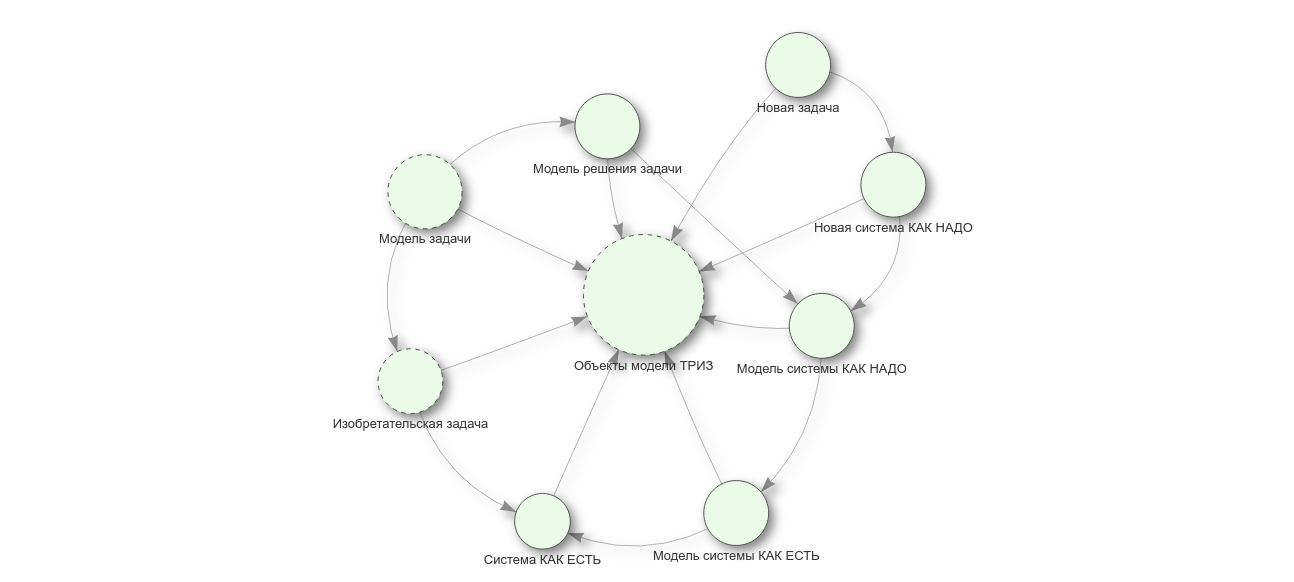
\includegraphics[width=.8\textwidth]{8.png}\\.
  Figure 8: Ontological chart \emph{Objects of a TRIZ model}
  \url{https://onto.devtas.ru/new?view=29e5aabb-996c-8fba-1554-b94dacb696ae} 
\end{center}
This chart shows that the \emph{system as it is} can contain an
\emph{inventive task}, can be transformed into a \emph{model of the system as
  it is}.  The \emph{task model} is derived from the \emph{inventive task} and
can be transformed into a \emph{model of task solutions}. The \emph{model of
  the system as it should be} can contain an \emph{model of task solution} and
can be transformed into a \emph{system as it should be} (synonymous with
\emph{new system}), which in turn may contain a \emph{new task}.

Each transition from one object of a TRIZ model to another is carried out by
appropriate TRIZ methods, which are described in the \emph{Methods in TRIZ}
ontology.  The current status of this
section\footnote{\url{https://triz-summit.ru/onto_triz/mod/metod/}} is given
below in the text of this report.

\textbf{Ontology \emph{Methods in TRIZ}}
\begin{itemize}
\item Ontology \emph{Methods of systems analysis brought to TRIZ}
  \begin{itemize}[noitemsep]
  \item Ontology \emph{MPV Analysis} 
  \item Ontology \emph{Function Value Analysis} (FVA) 
  \item \emph{Benchmarking} Ontology
  \item Ontology \emph{Parametric Analysis}
  \item Ontology \emph{RCA+ Analysis} 
  \item \emph{Ishikawa Diagram} Ontology
  \item Ontology \emph{Cause and effect analysis}
  \end{itemize}
\item Ontology \emph{Methods of systems analysis developed within TRIZ}
  \begin{itemize}[noitemsep]
  \item \emph{Functional Analysis} Ontology
  \item Ontology \emph{Element-Field Analysis}
  \item Ontology \emph{Component Analysis}
  \item Ontology \emph{Resource Analysis}
  \item Ontology \emph{Flow Analysis}
  \item Ontology \emph{Diversion Analysis}
  \item Ontology \emph{Structural Analysis}
  \item Ontology \emph{Analysis of the principle of action} 
  \item Ontology \emph{System Operator Analysis}
  \end{itemize}
\item Ontology \emph{Methods of system transformation}
  \begin{itemize}[noitemsep]
  \item Ontology \emph{Techniques of conflict resolution}
  \item Ontology \emph{Method of trial and error}
  \item Ontology \emph{Application of laws and trends of system evolution}
  \item Ontology \emph{Method of analogies}
  \item Ontology \emph{Unification of alternative systems}
  \end{itemize}
\item Ontology \emph{Methods of solving inventive tasks}
  \begin{itemize}[noitemsep]
  \item Ontology \emph{Principles of resolving contradictions}
  \item Ontology \emph{Connection of principles and methods of conflict
    resolution} 
  \item Ontology \emph{Table of application of conflict resolution techniques} 
  \item Ontology \emph{Element-Field transformations}
  \item Ontology \emph{Functionally-oriented search} (FOS)
  \item Ontology \emph{Ideal final result} (IFR)
  \end{itemize}
\item Ontology \emph{Methods of evaluation and development of concepts of
  system transformation}
  \begin{itemize}[noitemsep]
  \item Ontology of \emph{Supereffects}
  \item Ontology of \emph{Secondary Tasks}
  \item Ontology \emph{Methods of generalization of the solution found}
  \end{itemize}
\item Ontology \emph{Integral Methods of System Development}
  \begin{itemize}[noitemsep]
  \item \emph{ARIZ} Ontology
  \item Ontology \emph{Standards for solving inventive problems}
  \item \emph{TRIZ Analysis} ontology
  \item Ontology \emph{Linking laws and trends with TRIZ tools}
  \end{itemize}
\end{itemize}
In the future, the structure of the ontology \emph{Methods in TRIZ} will be
further clarified.

TRIZ projects life cycle includes 4 main stages:
\begin{itemize}[noitemsep]
\item identification of undesired effects and pre-project phase,
\item conceptual stage,
\item verification and
\item implementation.
\end{itemize}
In such a way \emph{TRIZ Project Activities} and \emph{TRIZ Project Life
  Cycle} correlate with the \emph{TRIZ models} cycle of system development and
solution of inventive tasks. We reproduce an extract from the TRIZ Ontology
table of contents, related to the \emph{TRIZ Model} ontology:

\textbf{Ontology \emph{TRIZ application areas}}
\begin{itemize}
\item Ontology \emph{Subjects of TRIZ application areas}
  \begin{itemize}[noitemsep]
  \item Ontology \emph{TRIZ in innovative entrepreneurship}
    \begin{itemize}[noitemsep]
    \item Ontology \emph{Analysis of the market from the perspective of
      contradictions and their resolution}
    \item Ontology \emph{MPV Analysis}
    \item Ontology \emph{Analysis of needs and their development directions}
    \end{itemize}
  \item Ontology \emph{TRIZ in the development of industrial enterprises}
  \item Ontology \emph{TRIZ in programming and information systems}
  \item Ontology \emph{TRIZ in art, literature and design}
  \item Ontology \emph{TRIZ in business}
  \item Ontology \emph{TRIZ in solving scientific problems}
  \item Ontology \emph{TRIZ in team development and social systems}
  \end{itemize}
\item Ontology \emph{Project activities based on TRIZ}
  \begin{itemize}[noitemsep]
  \item Ontology \emph{TRIZ in solving inventive problems}
  \item Ontology \emph{TRIZ in consulting activities}
  \item Ontology \emph{TRIZ in forecasting}
  \item Ontology \emph{Road Maps of TRIZ Projects}
  \item Ontology \emph{Life Cycle of a TRIZ Project}
  \end{itemize}
\end{itemize}

Thus, the theoretical basis and methods of TRIZ are directly related to
practical project activities using TRIZ in system development and solving
inventive tasks.

\subsection{Ontology \emph{Scientific Base of TRIZ}}

In the first fundamental publication on the subject of TRIZ by G.S. Altshuller
and R.B. Shapiro \emph{On the psychology of inventive
  creativity}\footnote{\foreignlanguage{russian}{Г.С. Альтшуллер, Р.Б. Шапиро
    «О психологии изобретательского творчества» в журнале Вопросы психологии,
    No 6 в 1956 году}.}, the authors refer to the laws of dialectics and to 
scientific research in the area of psychology of creativity.

As TRIZ developed as a scientific theory, the scientific basis for TRIZ
expanded: system approach, functional approach, evolutionary approach and
fundamental scientific approaches are at the heart of TRIZ.

With this, scientific approaches specific to TRIZ have also been developed
research conducted.

The ontology \emph{Scientific Base of TRIZ} is the basis for all of the
\emph{TRIZ Ontology} as a whole.

At present, in the Ontology \emph{Scientific Base of TRIZ} have been formed
the following sections:
\begin{itemize}[noitemsep]
\item Ontology \emph{Dialectics} 
\item Ontology \emph{System Approach} 
\item Ontology \emph{Functional Approach}
\item Ontology \emph{Evolutionary Approach}
\item Ontology \emph{Parametric Approach}
\item Ontology \emph{Model Approach}
\item Ontology \emph{Psychology of creative thinking}
\item Ontology \emph{TRIZ Approaches}
\item Ontology \emph{Information Funds on System Development}
\end{itemize}

\begin{center}
  \addpicture
  Figure 9. Reference to the ontological chart \emph{Scientific base of
    TRIZ}\footnote{\url{https://onto.devtas.ru/new?view=c38a00d7-e97c-9648-bbc2-2af7b21d5d0e}}
\end{center}

One of the sections of the ontology \emph{Scientific Base of TRIZ} is the
ontology \emph{Model approach}.  A model (fr. mod\'ele from Latin modulus --
measure, analogue, sample) is a system whose research serves as a means to
obtain information about another system; to present some real process, devices
or concepts.  A model is an abstract representation of reality in a given form
(e.g. in mathematical, physical, symbolic, graphic or descriptive form),
designed to represent certain aspects of this reality and allowing you to get
answers to the questions you are studying. [Wikipedia]

The sections of the ontology \emph{Scientific base of TRIZ} are published in
more detail on the website \url{https://triz-summit.ru/onto_triz/science/}.

\subsection{Function and Functional Analysis}

At its core, TRIZ relies on a functional approach. The concept of
\emph{Function} for TRIZ is one of the central concepts. The function is used
in many tools: functional value analysis, functional analysis, functionally
perfect modeling, functionally oriented search and others.

Ontologically, the concept of \emph{Function} [9] is linked to the Functional
Approach, options of function presentation, kinds and types (Figure 7).
\begin{center}
  \addpicture
  Figure 10. Ontological diagram \emph{Function}
\end{center}
A function can be represented in the form of a functional model (subject,
performer of the action, -- action aimed at changing the parameter, -- object
whose parameter is changed), as an element-field or, as a particular case,
as a sufield representation (Figure 7).
\begin{center}
  \addpicture
  Figure 11. Ontological diagram \emph{Type of a function}
\end{center}
Functions are subdivided by type (Figure 8) into useful and harmful functions,
as well as a separate group of useful functions with a disadvantage is singled
out in the ontology.  Shortcomings of useful functions include redundancy,
insufficiency, bad functions manageability or lack of the required function.

Functions are subdivided by kind of function depending on the system level:
system functions, subsystem and supersystem functions. Also as kind are
singled out element functions, as a representative of a subsystem, and
functions of objects in the environment, as a representative of the
supersystem.

\begin{center}
  \addpicture
  Figure 12. Ontological diagram \emph{System function}
\end{center}
The functions of the system determine the impact capabilities of the system
under consideration to other systems in the supersystem (Figure 9). The
\emph{main function} of the system is a function, for which the system was
created. The main function implements the purpose of the system in relation to
the supersystem [2]. An \emph{additional function} is a function that is not
necessary to support the core process, but which accompanies the main function
or helps to achieve it [2]. A \emph{latent function} is a function, which was
not envisaged by the system designer, but which may be performed by the system
based on the needs of the system user.

\begin{center}
  \addpicture
  Figure 13. Ontological diagram \emph{Function of an element}
\end{center}
The functions of an element determine the capabilities of the element in
question to impact on other elements of the subsystem or supersystem (Figure
10).  The element's functions are divided into main and auxiliary ones.
\emph{Main functions} are aimed at the impact on the target object of the
system under consideration.  An \emph{auxiliary function} is directed at a
subsystem element or at an element of the supersystem that is not the intended
target of the system under consideration. Functions of object of the
environment, the supersystem and subsystems are currently not classified in
the described ontology.

As mentioned earlier, the term "Function" is used in various TRIZ instruments.
At the time of writing this report, in the OSA system ontological charts of
\emph{Functional Analysis} are worked out [10].

Functional Analysis is part of the \emph{Methods of System Analysis} diagram
[11], see Figure 11.
\begin{center}
  \addpicture
  Figure 14: Ontological diagram \emph{Methods of systems analysis}
\end{center}
\begin{center}
  \addpicture
  Figure 15. Ontological diagram \emph{Functional analysis}
\end{center}
The ontological diagram \emph{Functional Analysis} (Figure 12) illustrates the
connection with the objectives of the analysis, the models of functional
analysis, the construction of rules and transformations by models, and also
shows two individual cases of functional analysis: functional analysis of a
system and functional analysis of a process.
\begin{center}
  \addpicture
  Figure 16. Ontological diagram \emph{Objectives of functional analysis}
\end{center}
The objectives (Figure 16) of the functional analysis include:
\begin{itemize}[noitemsep]
\item Identification and setting of tasks;
\item Search for resources within the system or in its surroundings;
\item Finding new system links;
\item Assessment of the functional model of the system for compliance with the
  requirements.
\end{itemize}
\begin{center}
  \addpicture
  Figure 17. Ontological diagram \emph{Models of Functional Analysis}
\end{center}
Functional analysis models (Figure 17) are selected based on the kind of
analysis. For the \emph{functional analysis of the system}, a functional model
of the system is selected that is built on the basis of a component-structural
model, indicating its interactions and their characteristics. For a
\emph{functional process model}, a model is being built, a particular case of
which is the \emph{flow model}.

Having reached the function in the ontological diagram of the Functional
Analysis of a system, the observer automatically enters the function diagram.
Thus, there is no need to redefine the characteristics of functions.

\subsection{Flow and Flow Analysis}

Based on the definition from Sushkov's glossary [2], \emph{Flow analysis} is
an analytical method and a tool that identifies deficiencies in the flow of
energy, substances and information in a technical system. Oleg Gerasimov [14]
describes Flow Analysis as an analysis of a technical systems based on the
identification of deficiencies in flows of energy, substances and information
within the technical system, its grey areas, bottlenecks, bifurcations,
various losses, etc.

Most of the subsequent work was carried out by Yuri Lebedev, who introduces a
definition of flow (previously lacking) as a dynamic component of a system,
specifying that \emph{Flows} in the technical system are specific components.
The main feature of the flow as a component is the distribution (in space and
time) of its parameters. The other (stationary) components of the sytem are
localised in space. Because of this difference, the flows extremely
uncomfortable fit within the functional approach. For this reason, a special
tool was developed -- \emph{flow analysis} (FA). Accordingly, it is proposed
to consider flow analysis as a specific, particular case of functional
analysis.

The construction of an ontological chart makes it possible to define flow
analysis more precisely, as well as the flow model in flow analysis. In
addition, to show the relationship of flow analysis to functional analysis and
other TRIZ concepts. With this goal two basic ontological charts were
constructed: first the ontological chart of \emph{flow analysis} and 
second the ontological chart of \emph{flow models}, as detailed below.
\begin{center}
  \addpicture
  Figure 18. Ontological diagram \emph{Flow analysis} top
  level\footnote{\url{https://onto.devtas.ru/new?view=e48bd4bd-3eba-c548-64da-73da1886f744}} 
\end{center}
You see, that the ontology map changes the understanding of the objectives of
flow analysis by passing on from the search for shortcomings to a more complex
goal where the search for shortcomings is just a special case.

\begin{center}
  \addpicture
  Figure 19: Ontological diagram \emph{Flow analysis}, part \emph{Rules
  to perform flow analysis}
\end{center}
As a result of the ontocards construction, the following definitions for flow
model and flow analysis are clarified.

\emph{Flow analysis} is a special case of functional analysis of processes and
serves two main purposes. First, the descriptive purpose is to establish
relationships and search for resources. Secondly, checking the flow for
compliance requirements and, as a result, the identification of useful,
harmful and parasitic flows, as well as their change. The rules for performing
flow analysis include rules of assessment of a flow model, rules of
construction of model of flows \emph{as they are}, rules of application of
patterns of the evolution of flows in technical systems, as well as rules for
building a model of flows based on the compliance with the requirements placed
on it. The results of applying these rules are models of the flows \emph{as
  they are} and \emph{as required}, as well as a list of tasks and
contradictions for the subsequent solution. Using techniques for changing
flows, such as searching for grey zones or bottlenecks, one can move from
a model of flows \emph{as they are} to a model of flows \emph{as required}.
\begin{center}
  \addpicture
  Figure 20. Ontological diagram \emph{model of 
  flows}\footnote{\url{https://onto.devtas.ru/new?view=aacb6c47-827e-b850-7872-978858d06d22}} 
\end{center}
To describe the model of flows a method of description is chosen (most often
graphical).  Then static flow components are defined, including the control
system, channel, receiver and source. The control system may be of two types:
pump or valve, and the source: source of potential or source of current.  An
important characteristic of flows in flow analysis is the flow content, i.e.
the determination what flows through the channel, substance, energy and
information.  Another key characteristic is utility of the flow,
distinguishing useful, harmful or parasitic flows. Most others characteristics
are selected during the analysis process depending on the objectives and the
content of the flow. Concerning the type of characteristic, the original
notion of \emph{flow functionality} has been changed to the \emph{utility of
  the flow}, as the functionality of the flow is related to its functions, the
utility with its value to the consumer.

The construction of ontological diagrams makes it possible to find grey areas
and not formalised parts of knowledge. Links with other knowledge related to
TRIZ are shown more clearly. The next steps may be: description of grey areas,
various rules for building models, algorithms, and also a matrix of techniques
for transition from the model (or system) \emph{as it is} to the model (or
system) \emph{as required}.  Renaming of terms to better represent the essence
of the described concept is also one of the advantages of this approach.

\subsection{RTV -- Creative Imagination Development}

The Creative Imagination Development (hereinafter referred to as RTV) -- is an
auxiliary course, the purpose of which is to develop a managed imagination and
the ability to overcome psychological inertia in the process of solution of
inventive tasks\footnote{\url{https://triz-summit.ru/onto_triz/rtv/}}.
\begin{center}
  \addpicture
  Figure 21. Ontological diagram \emph{Tools for the Development of Creative
    Imagination}
\end{center}
\textbf{Primary differences in the RTV course:}
\begin{itemize}
\item[1.] The development of the imagination is based on the conscious use of
  the laws of system development. Thus, the method of modeling with little men
  is based on one of the main trends in the development of systems -- increase
  the degree of dispersion of working bodies. In Gordon's Synectic empathy is
  used, that ignores this law and is therefore much weaker.
\item[2.] Fantasy is seen as a vector (\emph{jumping thought}): not only the
  length of the jump is important, but also its direction. The RTV course
  focuses primarily on developing a \emph{controlled fantasy}.
\item[3.] The sources of strong methods and techniques are TRIZ and the
  \emph{Register of SF ideas}.
\item[4.] The RTV course is related to TRIZ training: emphasis is on such
  exercises, that develop the qualities required for TRIZ application. At the
  same time the RTV course is related to the supersystem -- the development of
  strong thinking: the course also includes exercises that go beyond
  technology.
\item[5.] Training -- just like at TRIZ -- is conducted according to the
  principle: demand only what has been taught (i.e. not to expect the listener
  to do it on their own, to be able to generate strong ideas, F-ideas, without
  mastering laws, rules, methods).
\end{itemize}
The RTV course includes various methods to stimulate inventive thinking,
preceding the creation of TRIZ. The purpose of their study: develop components
of inventive thinking, such as flexibility, variability, use of analogies,
originality; the study of these methods allows to go deeper in understanding
the distinctive features of TRIZ.

\begin{center}
  \addpicture
  Figure 22: Ontological diagram \emph{Methods of psychological activation
  of inventive thinking}.
\end{center}
It seems essential to me that in the first half of the 1970th, in the classes
were found effective methods -- phantograms, modelling with small men, the
search for an X-factor on a planet, closed by \emph{conditional clouds}, the
\emph{golden fish}, the MTV operator\footnote{MTV (measure, time, value).},
etc. In my opinion, the creation of a \emph{multiscreen scheme of strng
  thinking} is particularly important\footnote{See G.S. Altshuller. About the
  history of the RTV course (in Russian).
  \url{https://www.altshuller.ru/rtv/rtv6.asp}}.
\begin{center}
  \addpicture  
  Figure 23. Ontological diagram \emph{Methods of Development of Creative 
    Imagination based on TRIZ}.
\end{center}
In the RTV course individual TRIZ instruments are included (system operator,
contradictions, IFR, MTV operator, method of small men) with a description of
the specifics of the application of these tools for developing a creative
imagination.
\begin{center}
  \addpicture
  Figure 24. Ontological diagram \emph{Connection with other sections of
    TRIZ}. 
\end{center}
The RTV course is the TRIZ section which is most closely related to the
psychology of inventive creativity. In formulating the definitions for some
terms materials on the psychology of creativity are used, among other on the
psychology of inventive creativity.

In particular, the terms \emph{Imagination}, \emph{Fantasy} and
\emph{Psychological Inertia} have definitions in which the concepts of
psychology and philosophy are used, and also definitions in which TRIZ
approaches are used.

\begin{center}
  \addpicture
  Figure 25. Ontological diagram \emph{Connection with the psychology of 
    inventive Creativity}.
\end{center}
As source of methods and techniques of the RTV Course are TRIZ and the
\emph{Register of Scientific Fantastic Ideas} (hereinafter referred to as the
\emph{Register of SF-Ideas}). Therefore, some terms of the Ontology of the RTV
course are linked to other sections of TRIZ Ontology in general.  For example,
the term \emph{System Operator}, \emph{MTV Operator}, \emph{Morphological
  analysis} are related to similar sections of TRIZ Ontology.

Preparing the programme for the RTV Course two lines in different directions
should be taken into account:
\begin{itemize}
\item It must be considered which components of inventive thinking are
  demanded for the inventive activities of a specific specialist (TRIZ
  training line);
\item at the same time the RTV course develops strong (inventive) thinking in
  in general, and is based on the laws of development of thinking (the line of
  thinking).
\end{itemize}
Currently in the ontology \emph{Course of Development of Creativity
  Imagination} methods of a "classical" course are included. Authors whose
work was considered creating the ontology: G.S. Altshuller, P.R. Amnuel,
M.S. Rubin, S.S. Litvin, B.L. Zlotin, A.V. Zusman, Yu.G. Tamberg,
M.N. Shusterman, G.I. Ivanov, I.N. Murashkovska, A.A. Nesterenko,
T.V. Klemihinina, S.V. Kreinina.

\textbf{Further work on the ontology \emph{Instruments of RTV}.}
\begin{itemize}
\item It is necessary to establish links between the RTV Course Ontology
  and other TRIZ ontologies.  
\item It is important to elaborate the transitions to a practical RTV course
  and diagnostic materials on developing inventive thinking.
\end{itemize}

\subsection{System operator and System operator analysis}.

The System Operator is part of the \emph{Systemic Approach} ontology.
\begin{center}
  \addpicture
  Figure 26. Ontological diagram \emph{Systemic approach}.
\end{center}
\begin{center}
  \addpicture
  Figure 27. A generalised chart \emph{Systemic Operator} from the Cmaps
  website. 
\end{center}
\begin{center}
  \addpicture
  Figure 28. Ontological chart from the OSA website.
\end{center}
\begin{center}
  \addpicture
  Figure 29.  Reference to the ontological chart \emph{Systemic
    Oerator}\footnote{\url{https://onto.devtas.ru/new?view=938811e9-76cb-6ef3-a2dc-aec74ff3d721}} 
\end{center}
The Ontology \emph{Systemic Operator Analysis} is part of the Ontology
\emph{Methods of system analysis}.
\begin{center}
  \addpicture
  Figure 30
\end{center}
Reference to the \emph{TRIZ} and \emph{Method of System Analysis} ontology
charts. 
\url{https://onto.devtas.ru/new?view=c38a00d7-e97c-9648-bbc2-2af7b21d5d0e}.

The following figure shows the relationship between the ontological chart
\emph{Methods of system analysis} and \emph{System Operator Analysis}.
\begin{center}
  \addpicture
  Figure 31
\end{center}
Reference to the ontology chart \emph{System Operator Analysis}:
\url{https://onto.devtas.ru/new?view=a83457ab-77bb-5466-0263-6f4bd5eb3b95}
\begin{center}
  \addpicture
  Figure 32.
\end{center}
Working with the \emph{System Operator} ontology allowed better to elaborate
the specifics of this TRIZ tool, its relation to the systemic approach, to the
laws of system evolution, the RTV course \emph{Development of creative
  imagination}. Areas of growth of methodology of building and using the
system operator have been identified, we started development work on analysis
of the variability of transitions on the screens of the system operator, on
the methodology of iterated changes to screens, on spatial system operator and
others directions of development of the system operator and system operator
analysis.

Next steps: 
\begin{itemize}
\item Complete the compilation of the Ontological charts \emph{Systemic
  Operator} and \emph{System Operator Analysis}.
\item Develop methods to apply the systemic operator to the solution of
  inventive tasks and to forecasting system development.
\item Highlight common aspects in the construction of ontological charts of
  various analysis methods from the \emph{System Analysis Methods} ontology.
\end{itemize}

\section{The TRIZ ontology project}

\subsection{Goals and objectives of the project}

The TRIZ ontology project was initiated in 2019 by a group of TRIZ
specialists: Andrey Kuryan, Valery Souchkov, Dmitry Kucheryavy, Mikhail Rubin,
Nikolai Shchedrin as part of the TRIZ Summit 2019 based on report [8].

The objectives of the project are:
\begin{itemize}
\item[] Regarding the existing TRIZ Glossary:
  \begin{itemize}[noitemsep]
  \item check the correctness of each term in the existing TRIZ Glossary;
  \item clarify the terms and definitions in the existing TRIZ Glossary;
  \item detect and eliminate gaps in the existing TRIZ Glossary.
  \end{itemize}
\item[] Regarding TRIZ in general:
  \begin{itemize}[noitemsep]
  \item improve the quality of TRIZ training and understanding;
  \item help avoid incorrect use and incorrect interpretation of TRIZ terms;
  \item avoid unnecessary introducing of new terms;
  \item identify discrepancies in the use of TRIZ terms;
  \item contribute to the development of a theory that can provide
    quantitative predictive power;
  \item help in integrating TRIZ with or within other domains.
  \end{itemize}
\item[] The project envisages:
  \begin{itemize}[noitemsep]
  \item[1)] Identification of key TRIZ concepts that are related to other
    concepts of TRIZ through various relationships.
  \item[2)] Development of ontological diagrams showing the links between by
    the concepts of TRIZ.
  \item[3)] Discussion of ontological diagrams in the circle of TRIZ
    specialists.
  \item[4)] Development of new definitions of TRIZ concepts based on TRIZ
    ontologies.
  \end{itemize}
\end{itemize}
The project is open, i.e., every TRIZ specialist can take part in the project,
including the development of ontological diagrams, discuss already existing
ones or definitions of TRIZ concepts.

\subsection{The OSA Website}
\begin{quote}  
  This part of the Russian original is skipped since the site
  \url{https://onto.devtas.ru/ts2o1} is in Russian and requires a registration
  specific to Russian naming rules.

  Note also that the links to \url{https://onto.devtas.ru} subpages cited
  below do not produce the pictures displayed in the paper.
\end{quote}

\subsection{The triz-summit.ru Website}

TRIZ Ontology is being developed using three tools.  A preliminary, general
picture of the specific ontological section is being prepared on a specialised
website \url{https://onto.devtas.ru/ts2o1}.
\begin{center}
  \addpicture
  Figure 40: An ontological chart of the top level ontology
\end{center}
These connections are then transferred to ontology charts in the OSA system,
which has already been mentioned above and can be found at this link
\url{https://onto.devtas.ru/new?view=c38a00d7-e97c-9648-bbc2-2af7b21d5d0e}

To improve the availability of developments under the TRIZ Ontology project
and the organization of discussions all information on the project is
published on the Summit website of TRIZ developers
\url{https://triz-summit.ru/onto_triz/}.

In this section we will briefly describe the content and role of this website
in the project ...
\begin{quote}
  This part is also skipped since it can be explored at the given website
  link, 
\end{quote}
All main pages with description of ontologies of different concepts are
constructed in approximately the same form. On the page is described:
\begin{itemize}[noitemsep]
\item the hierarchy of the given concept in the TRIZ Ontology,
\item the definition in terms of the glossary by V. Souchkov (translated into
  Russian)
\item Changes, additions or refinements. Proposal for a new definition.
\end{itemize}
Synonyms.  
\begin{itemize}[noitemsep]
\item A list and references to dependent terms and concepts is given. 
\item Ontological charts are provided with a link to the OSA website.
\end{itemize}
Here are some examples (only the links are given here).
\begin{itemize}[noitemsep]
\item Description of the Ontology \emph{Administrative contradiction
  (problematic situation)}
  \url{https://triz-summit.ru/onto_triz/science/triz_ap/invent/contradict/adm/}
\item Description of the \emph{System Operator} Ontology:
  \url{https://triz-summit.ru/onto_triz/science/sys/sys_op/}
\end{itemize}
If new concepts are introduced, a rationale for introducing a new term or
concept are prepared and published for discussion. For example, on the website
\url{https://triz-summit.ru/onto_triz/science/sys/sys_op/svayz/var/} the
rationale for introducing the concept of \emph{Variability of System
  Transitions} has been published. On this page 
\begin{itemize}[noitemsep]
\item a hierarchical path to this concept is given: Home $\to$ TRIZ Ontology
  $\to$ Ontology \emph{TRIZ Science Basics} $\to$ Ontology \emph{System
  Approach} $\to$ Ontology \emph{System Operator} $\to$ Ontology \emph{Links
  between screens}.
\item a brief description and examples of usage is provided.
\item the rationale for introducing this concept (tool, analysis elements,
  etc.) is given.
\item an illustrative material is published.
\end{itemize}
\begin{quote}
  Several figures are skipped.
\end{quote}
Next steps and plans for the future: 
\begin{itemize}[noitemsep]
\item Complete the structure of the TRIZ Ontology section on the website.
\item Update definitions of terms and links to ontological maps.
\item Organise feedback to discuss sections and terms of the \emph{TRIZ
  Ontology} and the project development in general.
\item Enter a classification index of TRIZ materials in accordance with the
  TRIZ ontology.
\item Correct the \emph{Icarus and Daedalus} system according to the TRIZ
  Ontology.
\item Develop a guidebook for the TRIZ Summit website in accordance with the
  index of TRIZ materials.
\end{itemize}

\subsection{How the project is organised}

\begin{quote}
  Note that all material on the sites described below are in Russian only.
\end{quote}
An open platform has been created for the implementation of the TRIZ Ontology
project.  It includes:
\begin{itemize}[noitemsep]
\item[1.] a separate OSA platform for the development and storage of
  ontological diagrams;
\item[2.] A \emph{TRIZ Ontology} section on the \url{https://triz-summit.ru}
  website (hereinafter referred to as the TRIZ Ontology website), where the
  descriptions of TRIZ Ontologies are located.
\end{itemize}
The following figure shows the structural diagram of the platform for Ontology
TRIZ.
\begin{center}
  \addpicture
  Figure 46. Platform structure of the TRIZ Ontology project
\end{center}
The following table describes the stakeholder structure and responsibilities
within the TRIZ Ontology project.
\begin{center}
  \begin{tabular}{|l|p{12cm}|}\hline
    Moderator & A TRIZ Ontology team member. He is responsible for creating
    tasks to develop parts of the ontology by experts, as well as to monitor
    performing these tasks. \\\hline    
    Expert & A TRIZ Ontology team member. He is responsible for creating
    ontological diagrams and their descriptions. \\\hline    
    Visitor & This is any person who is interested in the area of TRIZ
    knowledge in general and the TRIZ Ontology in particular. A visitor can
    study ontological diagrams and their descriptions on
    \texttt{triz-summit.ru}, accept to participate in discussions and express
    his opinions and ratings. \\\hline
  \end{tabular}
\end{center}
The TRIZ Ontology project website also contains a description of the project
and sections \emph{Instructions for project participants} and \emph{TRIZ
Ontology proposals}  \url{https://triz-summit.ru/onto_triz/proj/predl/}.

\begin{quote}
  Several pictures are skipped.
\end{quote}

\section{Conclusion}

Compiling a TRIZ ontology is a necessary step for the development of TRIZ
today. It is the foundation on which a new version of TRIZ knowledge should be
built.

It is impossible to create a TRIZ Ontology without the participation of a wide
range of TRIZ specialists.  The authors of the report encourage all interested
parties to engage in TRIZ Ontology project.

\section{References}
\begin{itemize}[leftmargin=18pt]
\item[1.] G.S. Altshuller. \foreignlanguage{russian}{Справка ТРИЗ-88} (TRIZ-88
  Overview).\\ \url{https://www.altshuller.ru/engineering/engineering16.asp}
\item[2.] V. Souchkov. Glossary of TRIZ and TRIZ-related terms.  ver. 1.2.
  MATRIZ-2018.\\
  \url{https://matriz.org/wp-content/uploads/2016/11/TRIZ-Glossary.pdf}
\item[3.] S. Litvin, V. Petrov, M. Rubin. \foreignlanguage{russian}{Основы
  знаний по ТРИЗ} (TRIZ body of knowledge). Version 1.0. from
  2007.\\ \url{https://triz-summit.ru/triz/metod/basics/1/203703/}
\item[4.] MATRIZ Regulations for Multi-Level Certification of TRIZ Users and
  Specialists.  MATRIZ, 2016.
\item[5.] N.N Khomenko. \foreignlanguage{russian}{ОТСМ-ТРИЗ} (OTSM-TRIZ).
  \url{https://otsm-triz.org/en}
\item[6.] M.S. Rubin. \foreignlanguage{russian}{Эволюционное системоведение}
  (Evolutionary system
  science).\\ \url{https://triz-summit.ru/triz/metod/evos/}
\item[7.] \foreignlanguage{russian}{Международная система оценки знаний и навыков ТРИЗ “Икар и
  Дедал”} (International assessment system for TRIZ knowledge and expertise
  "Ikarus and Daedalus").\\ \url{https://triz-summit.ru/certif/}
\item[8.] A. Kuryan, V. Souchkov, D. Kucharavy. Towards ontology of TRIZ.
  Proceedings of TRIZ Developers Summit 2019 Conference, Minsk, 2019.\\
  \url{https://triz-summit.ru/confer/tds-2019/articles/it/}
\item[9.] {\small 
  \url{https://triz-summit.ru/onto_triz/analysis/fa/model_fa/func_syst_model/func/} }
\item[10.] \url{https://triz-summit.ru/onto_triz/analysis/fa/}
\item[11.] \url{https://triz-summit.ru/onto_triz/analysis/}
\item[12.] \url{https://devtas.ru/docs/}
\item[13.] \url{http://tas-project.ru/}
\item[14.] O. Gerasimov. \foreignlanguage{russian}{Потоковый Анализ} (Flow
  Analysis). NPK course material "TRIZ 100", Module 2. 
\end{itemize}
\end{document}
